\section{Сонгосон технологи}
\subsection{React \& Next.js}
\subsubsection{Declarative}
React нь хэрэглэгчийн интерактив интерфейс бүтээхийг хялбарчилдаг. Aппликейшны state бүрд зориулсан энгийн бүтэц зохион байгуулахаас гадна, React нь өгөгдөл өөрчлөгдөхөд яг зөв компонентоо өөрчлөн рендер хийдэг. Declarative бүтэц нь кодыг тань debug хийхэд хялбар болгохоос гадна, ажиллагаа нь илүү тодорхой болдог.

\subsubsection{Компонент-д тулгуурласан}
Бие даан state-ээ удирддаг маш энгийн компонент бичиж, эдгээрийг хольж найруулан нарийн бүтэцтэй хэрэглэгчийн интерфейс бүтээх боломжтой. Компонентийн логик нь тэмплэйтээр бус JavaScript-ээр бичигддэг учраас өгөгдлийг апп хооронд хялбар дамжуулж, DOM-оос state-ээ тусад нь байлгаж чадна.

\subsubsection{Next.js}
Netflix, TikTok, Hulu, Twitch, Nike гэсэн орчин үеийн аваргууд ашигладаг энэхүү орчин үеийн фрэймворк нь React технологи дээр үндэслэгдсэн бөгөөд Frontend, Backend хоёр талд хоёуланд нь ажилладаг веб аппуудыг хийх чадвартайгаараа бусдаасаа давуу юм. Next.js-ийн үндсэн дизайн нь клиент болон сервер талын аль алиных давуу талыг ашиглаж чаддаг, ямар нэг дутагдалгүй веб сайтыг яаж хамгийн хурдан хялбар бүтээх вэ гэдгийг бодож тусгасан байдаг. Next.js нь сервер талд react компонентуудыг рендерлэн энгийн html, css, json файл болгон хувиргах замаар ажилладаг бөгөөд 2020 оноос олон нийтэд танигдсан JAMStack технологи болон статик сайт, автоматаар статик хуудас үүсгэх, CDN deployment, сервергүй функц, тэг тохиргоо, файлын системийн рүүтинг (PHP-ээс санаа авсан), SWR (stale while revalidate), сервер талд рендерлэх зэрэг асар олон орчин үеийн шинэхэн технологиудыг бүгдийг хийж чаддаг анхны бүрэн веб фрэймворк гэж хэлж болно.

\subsection{Ethereum блокчэйн}
Төвлөрсөн бус, блокчэйн дээр суурилсан программуудыг хангамжийн платформ анх Ethereum-ийг 2013 онд программист Vitalik Buterin бичсэн бөгөөд 2015 онд олон нийтэд анх танилцуулагдсан юм. Ethereum нь бусад койныг бодвол зөвхөн арилжааны бус тус платформыг ашиглан smart contract буюу ухаалаг гэрээ үүсгэх боломжтой. Энэ нь энгийнээр хөгжүүлэгчдэд төвлөрсөн бус хэрэглээний программуудыг бүтээх, ажиллуулах боломжийг олгодог.

\subsection{Hardhat}
Hardhat нь ухаалаг гэрээг хөгжүүлэх орчин юм. Энэ нь Ethereum ухаалаг гэрээг бичих, туршихаас эхлээд байршуулах, дибаг хийх хүртэлх бүх амьдралын мөчлөгийг хөнгөвчлөх зорилготой юм. Hardhat нь Ethereum Virtual Machine (EVM) дээр бүтээгдсэн бөгөөд Ethereum, Polygon, Avalanche болон бусад EVM-тэй нийцтэй блокчэйнүүдийг дэмждэг.

\subsection{Wagmi}
Wagmi нь блокчэйнтэй ажиллахад шаардлагатай бүх зүйлийг агуулсан React Hook-ийн цуглуулга юм. Wagmi нь крифто түрийвч холбох, мэдээллийг авах, ухаалаг гэрээтэй харилцах гэх мэт үйлдлүүдийг хөнгөвчлөх боломжийг олгодог.

\subsection{IPFS \& Pinata}
IPFS буюу Interplanetary File System нь peer-to-peer сүлжээн дэх файлуудыг хадгалах, хуваалцахад зориулагдсан төвлөрсөн бус протокол юм. Үндсэндээ IPFS нь файлуудыг жижиг хэсгүүдэд хувааж, сүлжээний олон зангилаанд хадгалдаг. Энэ нь файлуудыг нэг байршилд хадгалдаггүй, харин сүлжээгээр тарааж байршуулдаг.
Pinata нь төвлөрсөн бус бичиг баримт хадгалалтын сүлжээ болох Interplanetary File System (IPFS) дээр бүтээгдсэн үйлчилгээ юм. Pinata нь хөгжүүлэгчид болон хэрэглэгчдэд IPFS сүлжээнд өгөгдөл хадгалах, уншихад хялбар болгодог. Энэ нь IPFS дээр хадгалагдсан файлуудыг байршуулах, удирдах, хандахад зориулсан API болон бусад хэрэгслээр хангаснаар IPFS-тэй харилцах үйл явцыг хялбаршуулдаг.

\subsection{Lit Protocol}
Lit Protocol нь өөр өөр талууд эсвэл программуудын хооронд аюулгүй, хувийн харилцаа холбоо, өгөгдөл дамжуулах боломжийг олгодог төвлөрсөн бус сүлжээний протокол юм. Энэ нь одоо байгаа блокчэйн болон төвлөрсөн бус хадгалалтын шийдлүүдийн дээр нууцлал, хандалтын хяналтын давхаргыг хангах зорилготой юм.

Lit Protocol-н хэд хэдэн гол технологи, ойлголтууд:
\begin{itemize}
   \item  End-to-End Шифрлэлт: Протокол нь талуудын хооронд хуваалцсан өгөгдөл нь нууц хэвээр үлдэж, зөвхөн хүссэн хүлээн авагчид хандах боломжтой байхын тулд төгсгөлөөс төгсгөл хүртэл шифрлэлтийг ашигладаг.
   \item  Хандалтын хяналтын нөхцөлүүд: Lit Protocol нь хандалтын хяналтын нөхцөлийн тухай ойлголтыг танилцуулсан бөгөөд энэ нь хэн тодорхой өгөгдөлд хандах эсвэл тодорхой үйлдлийг гүйцэтгэх боломжтой болохыг тодорхойлдог криптограф нотолгоо юм. Эдгээр нөхцөлүүд нь төвлөрсөн бус байдлаар хэрэгжиж, төвлөрсөн эрх мэдлийн хэрэгцээг арилгадаг.
   \item Төвлөрсөн бус таних тэмдэг: Протокол нь аюулгүй харилцаа холбоо, мэдээлэл солилцох үйл ажиллагаанд оролцож буй талуудыг төлөөлөхийн тулд Ethereum хаяг эсвэл блокчэйнд суурилсан бусад таних тэмдэг зэрэг төвлөрсөн бус таних тэмдгийг ашигладаг.
\end{itemize}

Энэхүү судалгааны ажлын хүрээнд хэрэглэгчийн байршуулсан файлуудыг шифрлэх, файлуудад хандах хандалтыг хянахад найдвартай, төвлөрсөн бус шийдлээр хангах зорилгоор Lit Protocol-ийг сонгосон. Lit Protocol-тэй нэгтгэснээр систем нь файлуудыг найдвартай хадгалж, хандалтын хяналтын тодорхой нөхцөөл дээр үндэслэн зөвхөн эрх бүхий этгээдэд хандах боломжтой.

\newpage
\section{Хөгжүүлэлт}

\subsection{Хөгжүүлэлтийн орчныг бэлдэх}
Энэхүү судалгааны ажлын практик хэсэгт би NextJS, Hardhat, Pinata, Wagmi, Tailwind CSS зэргийг ашиглан хөгжүүлэлт хийх билээ. NextJS нь монолитик төсөл хийхэд тохиромжтой ба төслийн ухаалаг гэрээ хөгжүүлэлт, клайнт талуудыг нэг repository-д хадгалж байгаа. Version Control System-ээр Github-г сонгосон юм. Кодын фолдер бүтэц нь дараах байдлаар байна.

\begin{figure}[h]
	\centering
	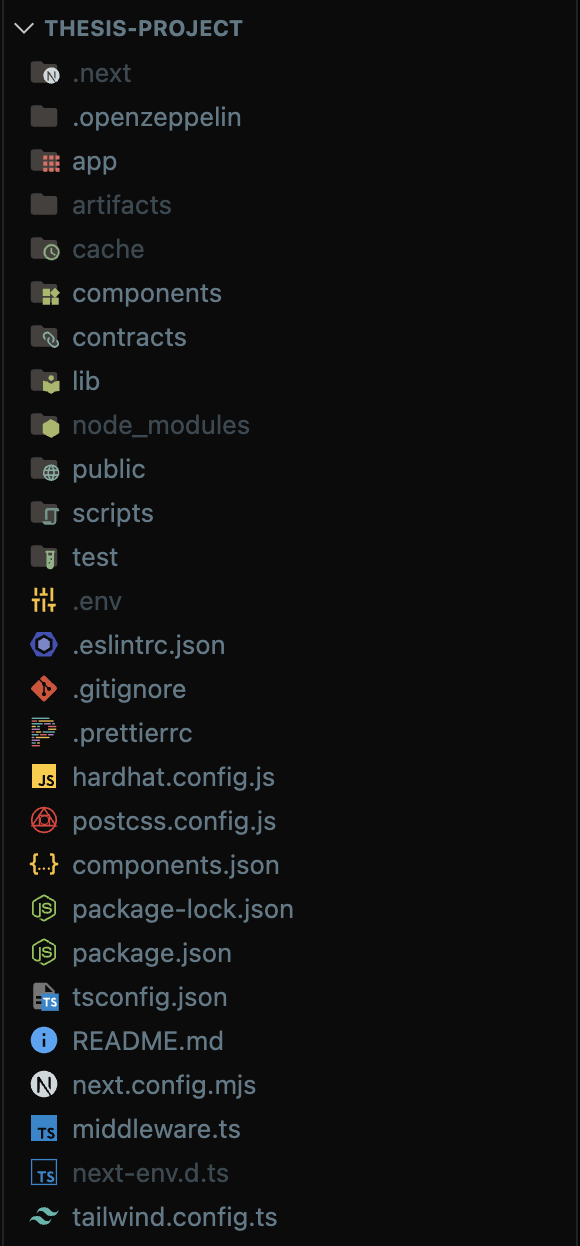
\includegraphics[scale=0.3]{src/images/folder-structure.png}
	\caption{Фолдерийн бүтэц}
\end{figure}

\begin{itemize}
	\item \textbf{components} - React компонентууд
	\item \textbf{lib} - Хэрэглэгчийн талын шаардлагатай код туслах функцууд
	\item \textbf{app} - NextJS дээрх хуудаснууд
	\item \textbf{public} - Статик зураг, файлууд
	\item \textbf{scripts} - Ухаалаг гэрээний хөгжүүлэлтийн холбоотой  javascript файлууд
	\item \textbf{contracts} - Ухаалаг гэрээний файлууд
\end{itemize}

\subsection{Ухаалаг гэрээн хөгжүүлэлт}
Миний төсөл нэг ухаалаг гэрээнээс бүтнэ. Уг ухаалаг гэрээ нь цахим файлууд болон тэдгээртэй холбоотой лицензүүдийг төлөөлдөг Файл ба Лиценз гэсэн хоёр бүтцийг тодорхойлсон.
Файл бүтэц  нь id, эзэмшигчийн хаяг, файлын нэр, тайлбар, ангилал, файлын хэш, үүсгэсэн хугацааны  зэрэг атрибутуудыг агуулна.
Лиценз бүтэц нь лицензийн дугаар, эзэмшигчийн хаяг, файлын нэр, тайлбар, ангилал, файлын хэш, үүсгэсэн хугацааны  зэрэг атрибутуудыг агуулна.
Мөн дараах функцүүдтэй:

\begin{itemize}
	\item \textbf{createFile}: Цахим баримт бичгийн мэдээллийг бичих
	\item \textbf{issueLicense}: Лицензийн мэдээллийг бичих
	\item \textbf{getAllPublicFiles}: Оруулсан бүх цахим баримт бичгийн авах
	\item \textbf{getAllUserFiles}:  Хэрэглэгчийн оруулсан цахим баримт бичгүүдийг авах
	\item \textbf{getAllUserLicenses}: Хэрэглэгчийн эзэмшиж буй лицензүүдийг авах
	\item \textbf{validateLicense}: Лицензийн дугаараар лицензийг шалгах
	\item \textbf{getPublicFileById}: Цахим баримт бичгийг  авах id-гаар нь авах
	\item \textbf{getMarketplaceFiles}: Лиценз авах боломжтой цахим баримт бичгүүдийг авах
	\item \textbf{generateUniqueLicense}: Лицензд өвөрмөц дугаар бий болгох
\end{itemize}

\subsection{Ухаалаг гэрээг блокчэйнд байршуулах}
\lstinputlisting[language=TypeScript,caption=deploy,basicstyle=\linespread{0.8}\ttfamily,frame=single]{src/code/deploy.js}

\subsection{Хэрэглэгч талын хөгжүүлэлт (Front-end)}
Уг код нь хэрэглэгчийн оруулах цахим баримт бичгийн мэдээллийг блокчэйнд бичнэ.
\lstinputlisting[language=TypeScript, caption=Блокчэйнд бичих,basicstyle=\linespread{0.8}\ttfamily,frame=single]{src/code/writeFile.ts}

Энэ функц нь хэрэглэгчийн оруулсан баримт бичгийг IPFS-д байршуулна.
\lstinputlisting[language=TypeScript, caption=Файл IPFS-д  байршуулах,basicstyle=\linespread{0.8}\ttfamily,frame=single]{src/code/uploadIpfs.ts}

Уг код нь хэрэглэгчийн оруулсан цахим баримт бичгүүдийн мэдээллийг блокчэйнээс уншина.
\lstinputlisting[language=TypeScript, caption=Блокчэйнээс унших,basicstyle=\linespread{0.8}\ttfamily,frame=single]{src/code/getUserFiles.ts}


\pagebreak
\subsection{Үр дүн}
Төслийн практик ажлын үр дүнд бүтээгдсэн  системийн интерфейс дараах байдлаар харагдана.
\begin{figure}[h!]
	\centering
	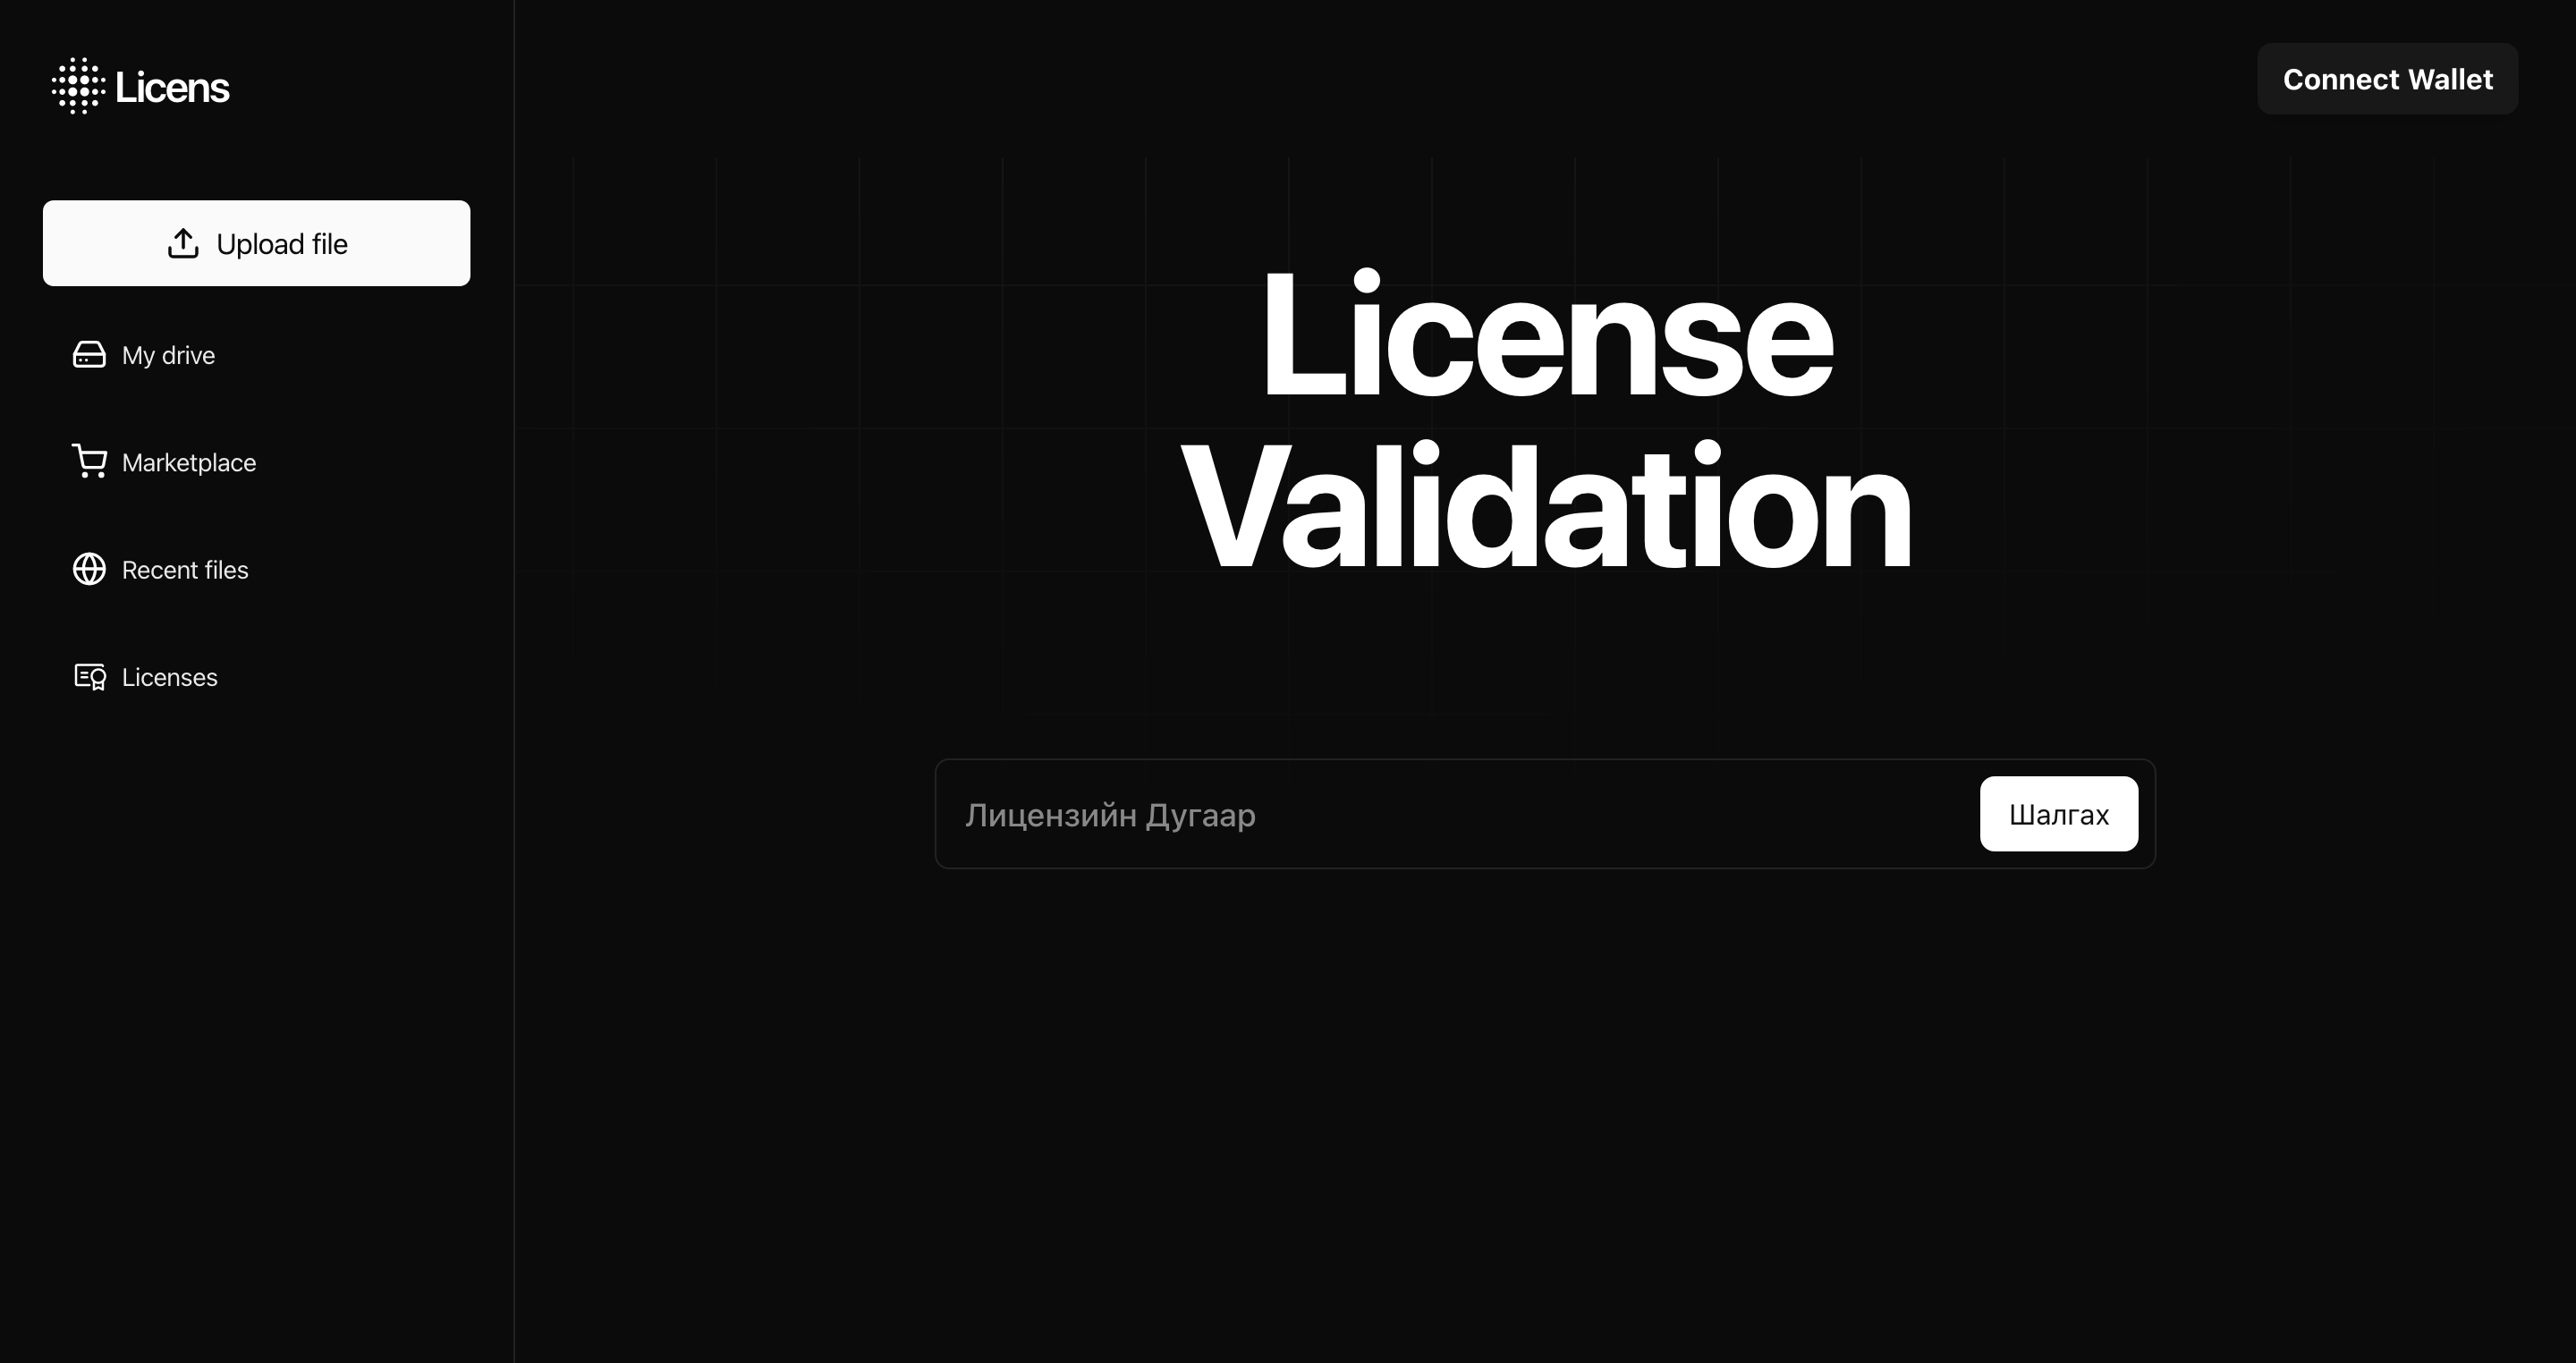
\includegraphics[scale=0.155]{src/images/homepage.png}
	\caption{Нүүр хуудас}
\end{figure}

\begin{figure}[h!]
	\centering
	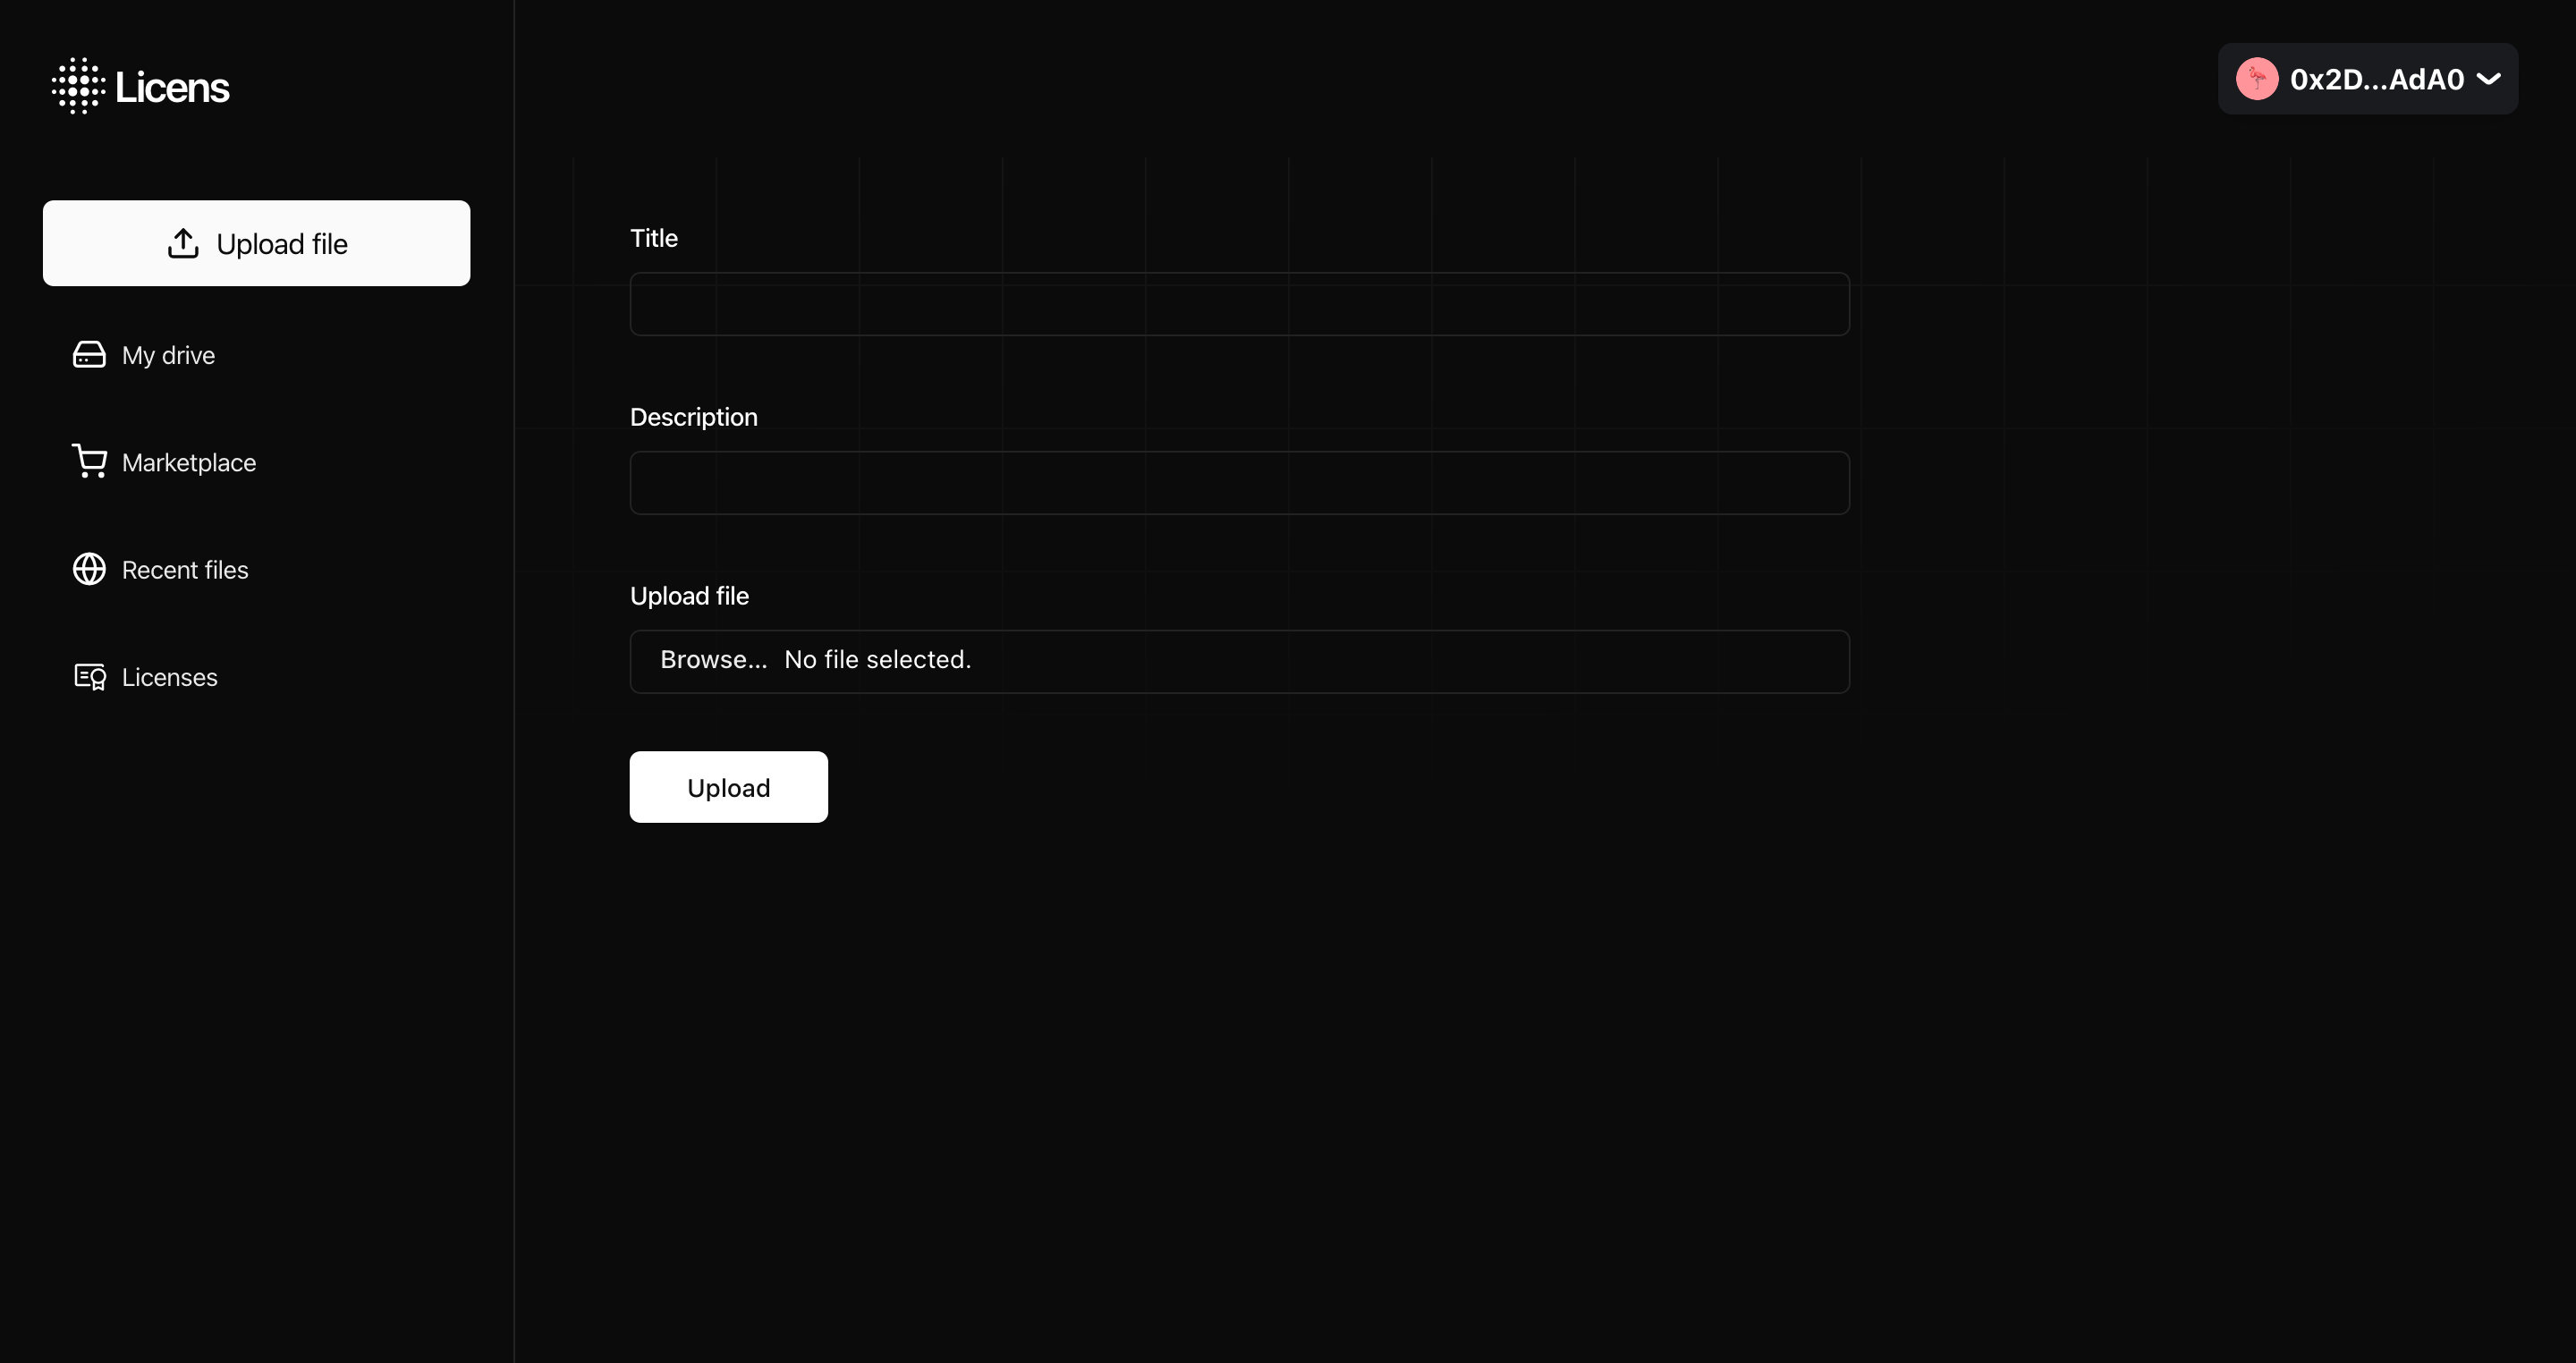
\includegraphics[scale=0.155]{src/images/upload-page.png}
	\caption{Цахим бичиг баримт оруулах}
\end{figure}

\begin{figure}[h!]
	\centering
	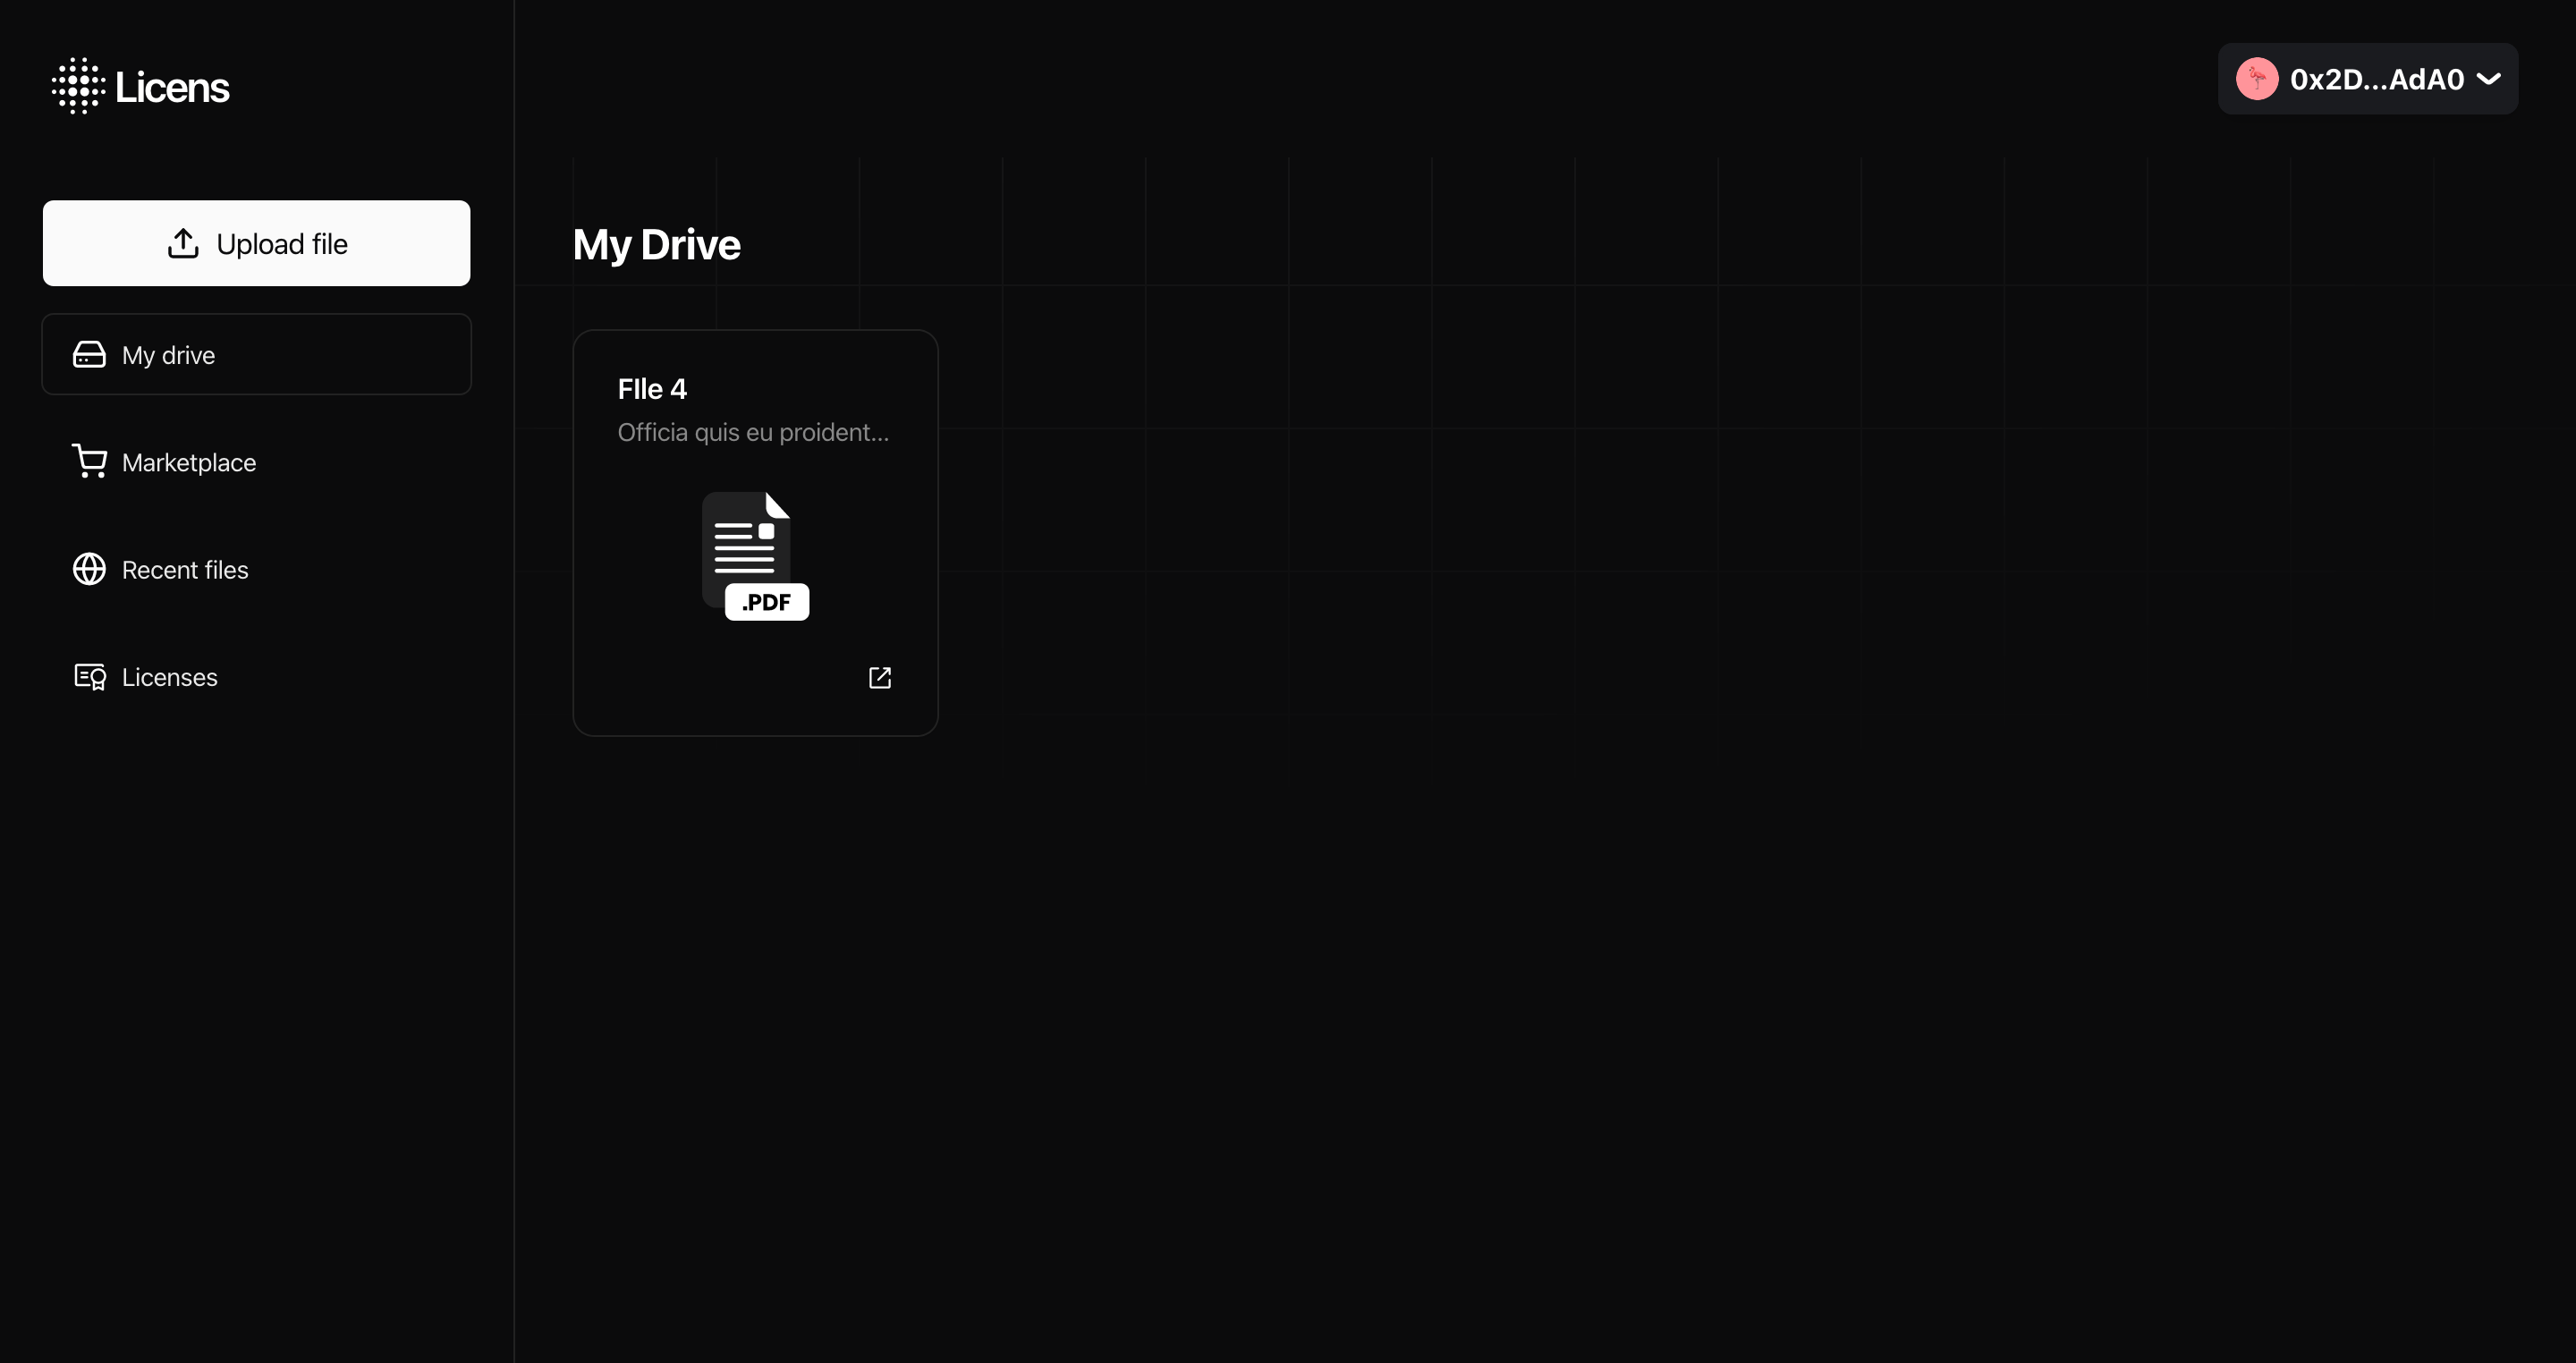
\includegraphics[scale=0.165]{src/images/drive-page.png}
	\caption{}
\end{figure}

\begin{figure}[h!]
	\centering
	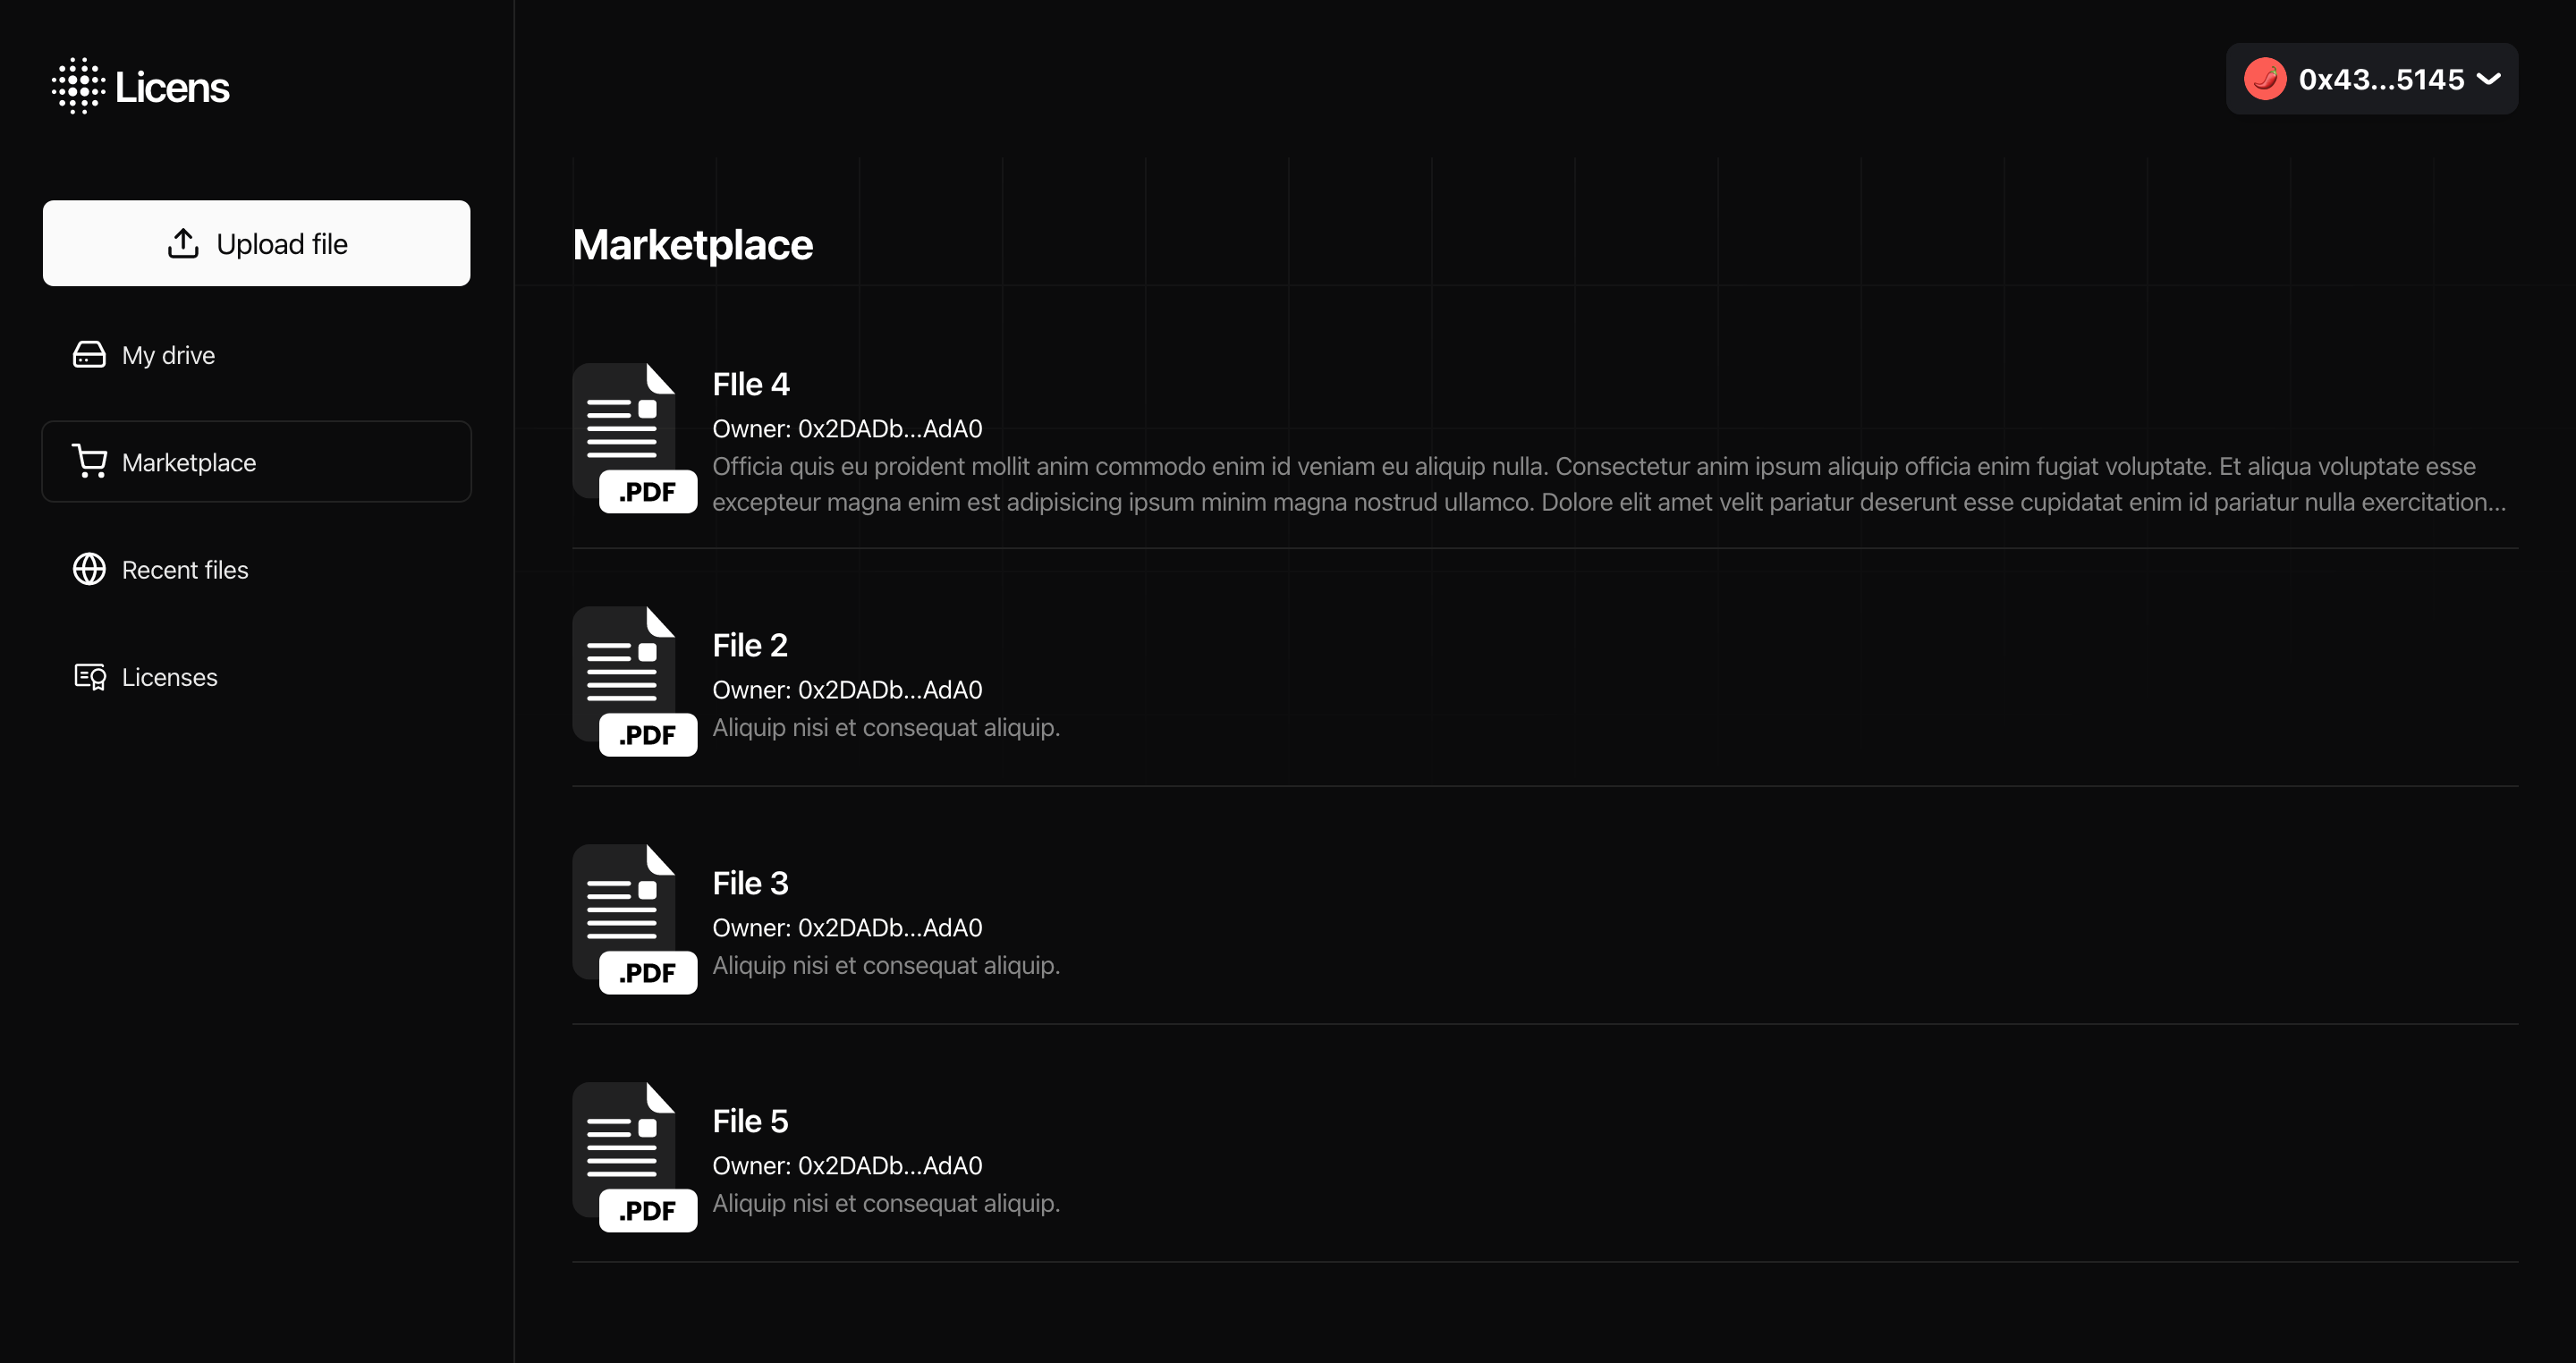
\includegraphics[scale=0.165]{src/images/marketplace-page.png}
	\caption{}
\end{figure}

\begin{figure}[h!]
	\centering
	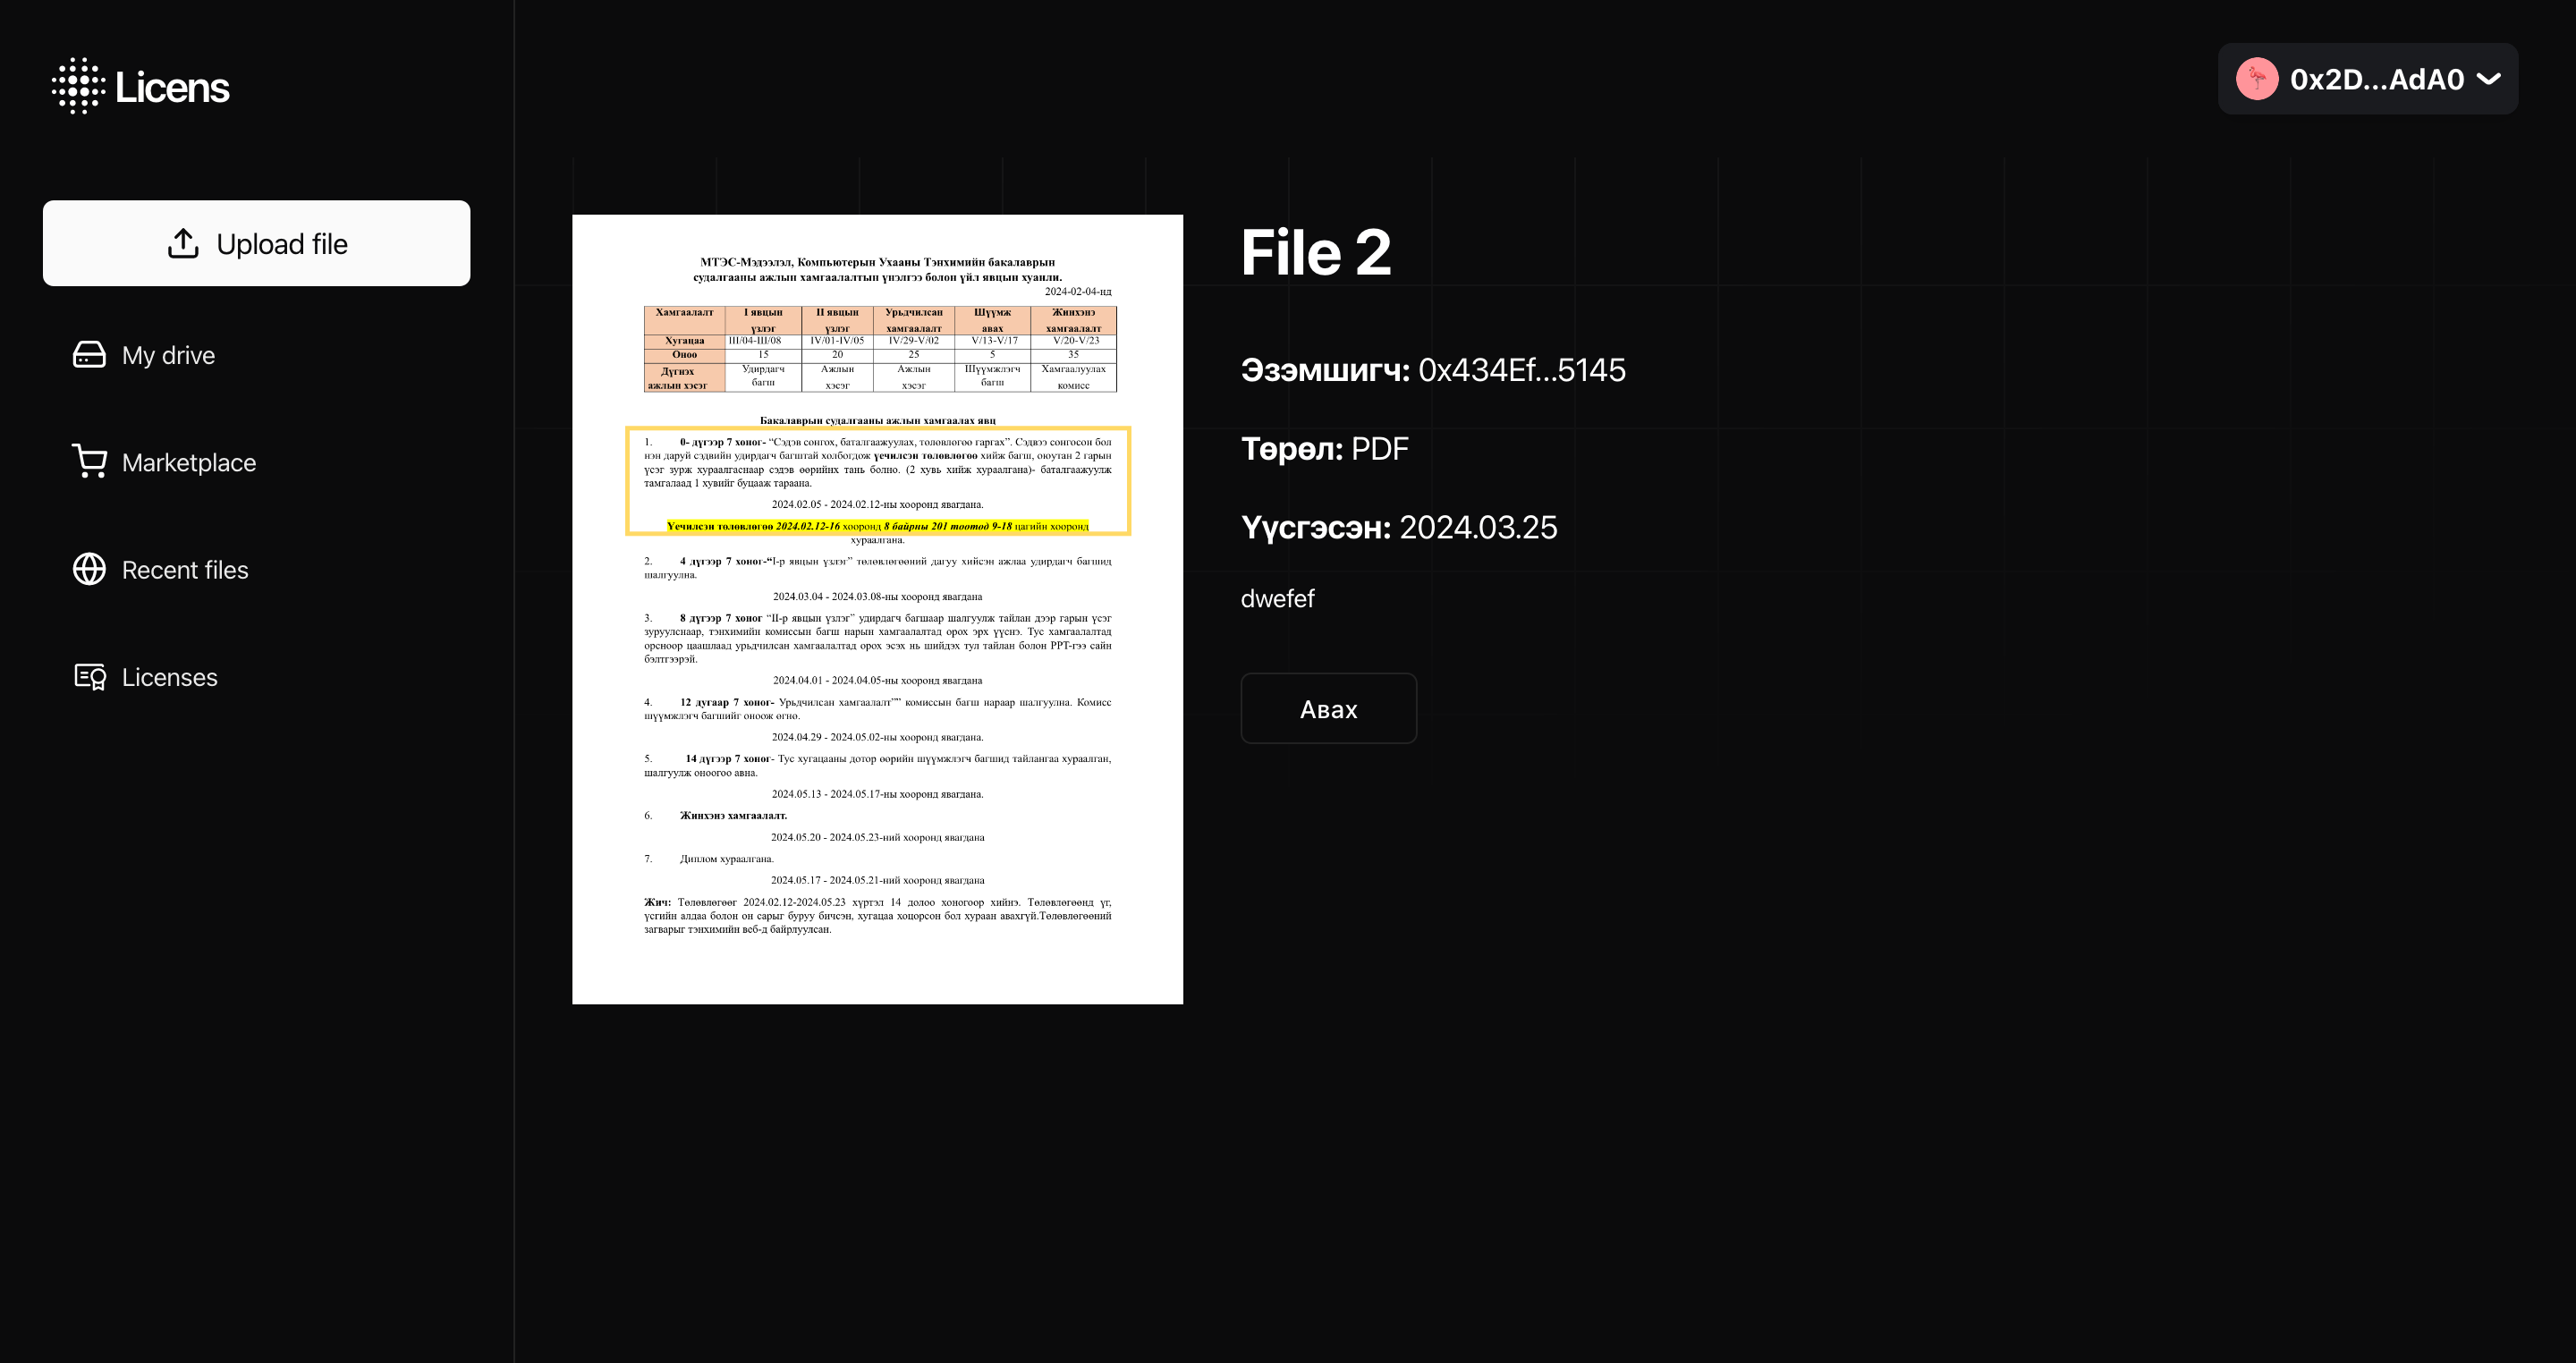
\includegraphics[scale=0.165]{src/images/file-page.png}
	\caption{}
\end{figure}